\section{Исследовательский раздел}
%В этом разделе представлены параметры технического устройства, на котором выполнялись измерения времени работы проектируемого приложения, а также результаты самих измерений.

\subsection{Постановка исследования}

Целью исследования является проведение анализа зависимости времени работы алгоритма составления турнирного расписания от количества команд, вступающих в турнир на строне базы данных.

\subsection{Технические характеристики}

Исследование проводилось на устройстве со следующими техническими характеристиками:

\begin{itemize}
	\item операционная система Window 10 Home Single Language;
	\item память 8 Гб;
	\item процессор 11th Gen Intel(R) Core(TM) i7-1165G7 2.80 ГГц, 4 ядра.
\end{itemize}

\subsection{Результаты исследования}

Для исследования зависимости времени составления расписания, использовалось четное количество команд. Количество команд менялось от 10 до 100 с шагом 10. Результаты исследования представлены в таблице \ref{table:time}.

\begin{table}[H]
	\begin{center}
		\caption{Результаты замеров времени}
		\begin{tabular}{|c|c|}
			\hline
			Количество команд & Время составления расписания \\
			\hline
			2 & 0.274000 \\
			\hline
			10 & 1.513000 \\
			\hline			
			20 & 4.714000 \\
			\hline			
			30 & 11.359000 \\
			\hline			
			40 & 21.928000 \\
			\hline			
			50 & 45.710000 \\
			\hline			
			60 & 67.000000 \\
			\hline			
			70 & 125.247000 \\
			\hline			
			80 & 174.082000 \\
			\hline			
			90 & 200.249000 \\
			\hline			
			100 & 218.990000 \\
			\hline			
		\end{tabular}
		\label{table:time}
	\end{center}
\end{table}

На рисунке \ref{fig:research} приведен график зависимости времени составления от числа команд.
\begin{figure}[h]
	\centering
	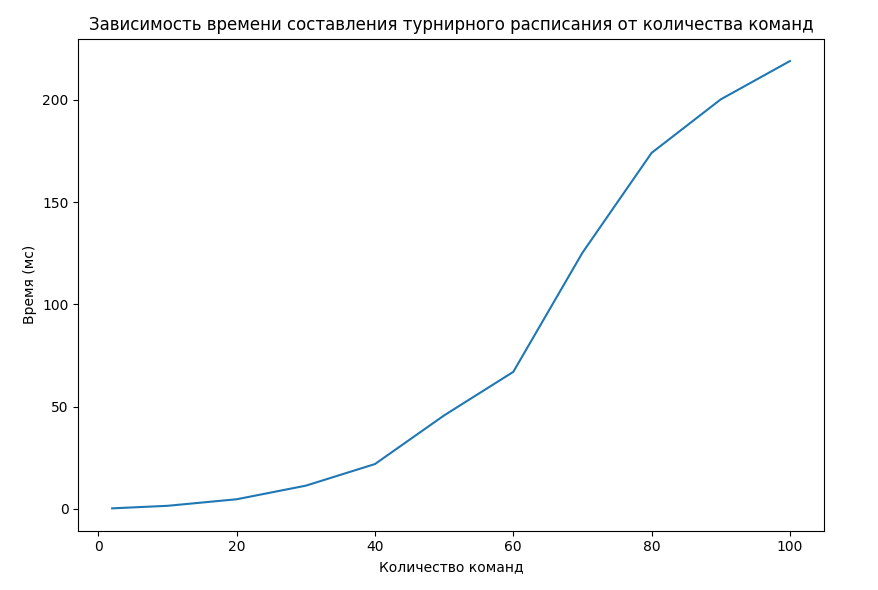
\includegraphics[width=0.9\textwidth]{img/research.png}
	\caption{График зависимости времени составления от числа команд}
	\label{fig:research}
\end{figure}

\subsection*{Вывод}
Из проведенного исследования можно сделать вывод, что время составления расписания линейно зависит от количества команд в турнире.